\documentclass{standalone}
\usepackage{tikz}

\begin{document}
  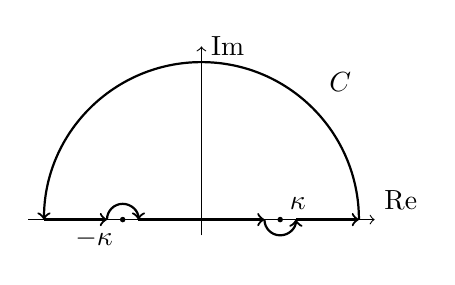
\begin{tikzpicture}
    \draw[->] (-2.2, 0) -- (2.2, 0) node[above right] {Re};
    \draw[->] (0, -0.2) -- (0, 2.2) node[right] {Im};
    \draw[thick, <-] (-2, 0) arc[start angle=180, end angle=0, radius=2];
    \draw[thick, ->] (-2, 0) -- (-1.2, 0);
    \draw[thick, ->] (-0.8, 0) -- (0.8, 0);
    \draw[thick, ->] (1.2, 0) -- (2, 0);
    \draw[thick, ->] (-1.2, 0) arc[start angle = 180, end angle = 0, radius=0.2];
    \draw[thick, ->] (0.8, 0) arc[start angle = 180, end angle = 360, radius=0.2];
    \node[above right] at (1.5, 1.5) {$C$};
    \fill (1, 0) circle(1pt) node[above right] {$\kappa$};
    \fill (-1, 0) circle(1pt) node[below left] {$-\kappa$};
  \end{tikzpicture}
\end{document}
